% !TeX spellcheck = en_GB
% ***************************************************** %
\section{Experiments and results discussion}\label{sc:exp}
% ***************************************************** %

%\begin{table}
%\caption[]{Hyper-parameters}
%\label{tab:hyper-params}
%\[
%\begin{array}{l}
%\beta=0.9 \\
%\end{array}
%\]
%\end{table}

%\begin{figure}
%\centering
%\includegraphics[width=0.3\textwidth]{../py/test.pdf}
%\end{figure}

% df.to_latex

To test the efficiency the algorithms, a benchmark of six datasets retrieved from \href{https://www.csie.ntu.edu.tw/~cjlin/libsvmtools/datasets/}{LIBSVM}.

First the six algorithms are tested on a fixed number of epochs, \texttt{bib2} set the value to \num{200}, so we do the same. We keep track of the objective function value for every epoch and the running time that every epoch took; our aim is to show how the value decreases on every epoch and the running time that takes.

Once we have the algorithms performance at different step-size values, a fine-tuning of the hyper-parameter is done in order to obtain the best solver for every dataset based on the accuracy score. For a better comparison, the L-BFGS, Conjugate Gradient and Newton-CG algorithms are also tested.

\begin{figure}
\centering
% diabetes
\subfloat[][\emph{Diabetes dataset}\label{subfig:diab-diagnostic}]%
	{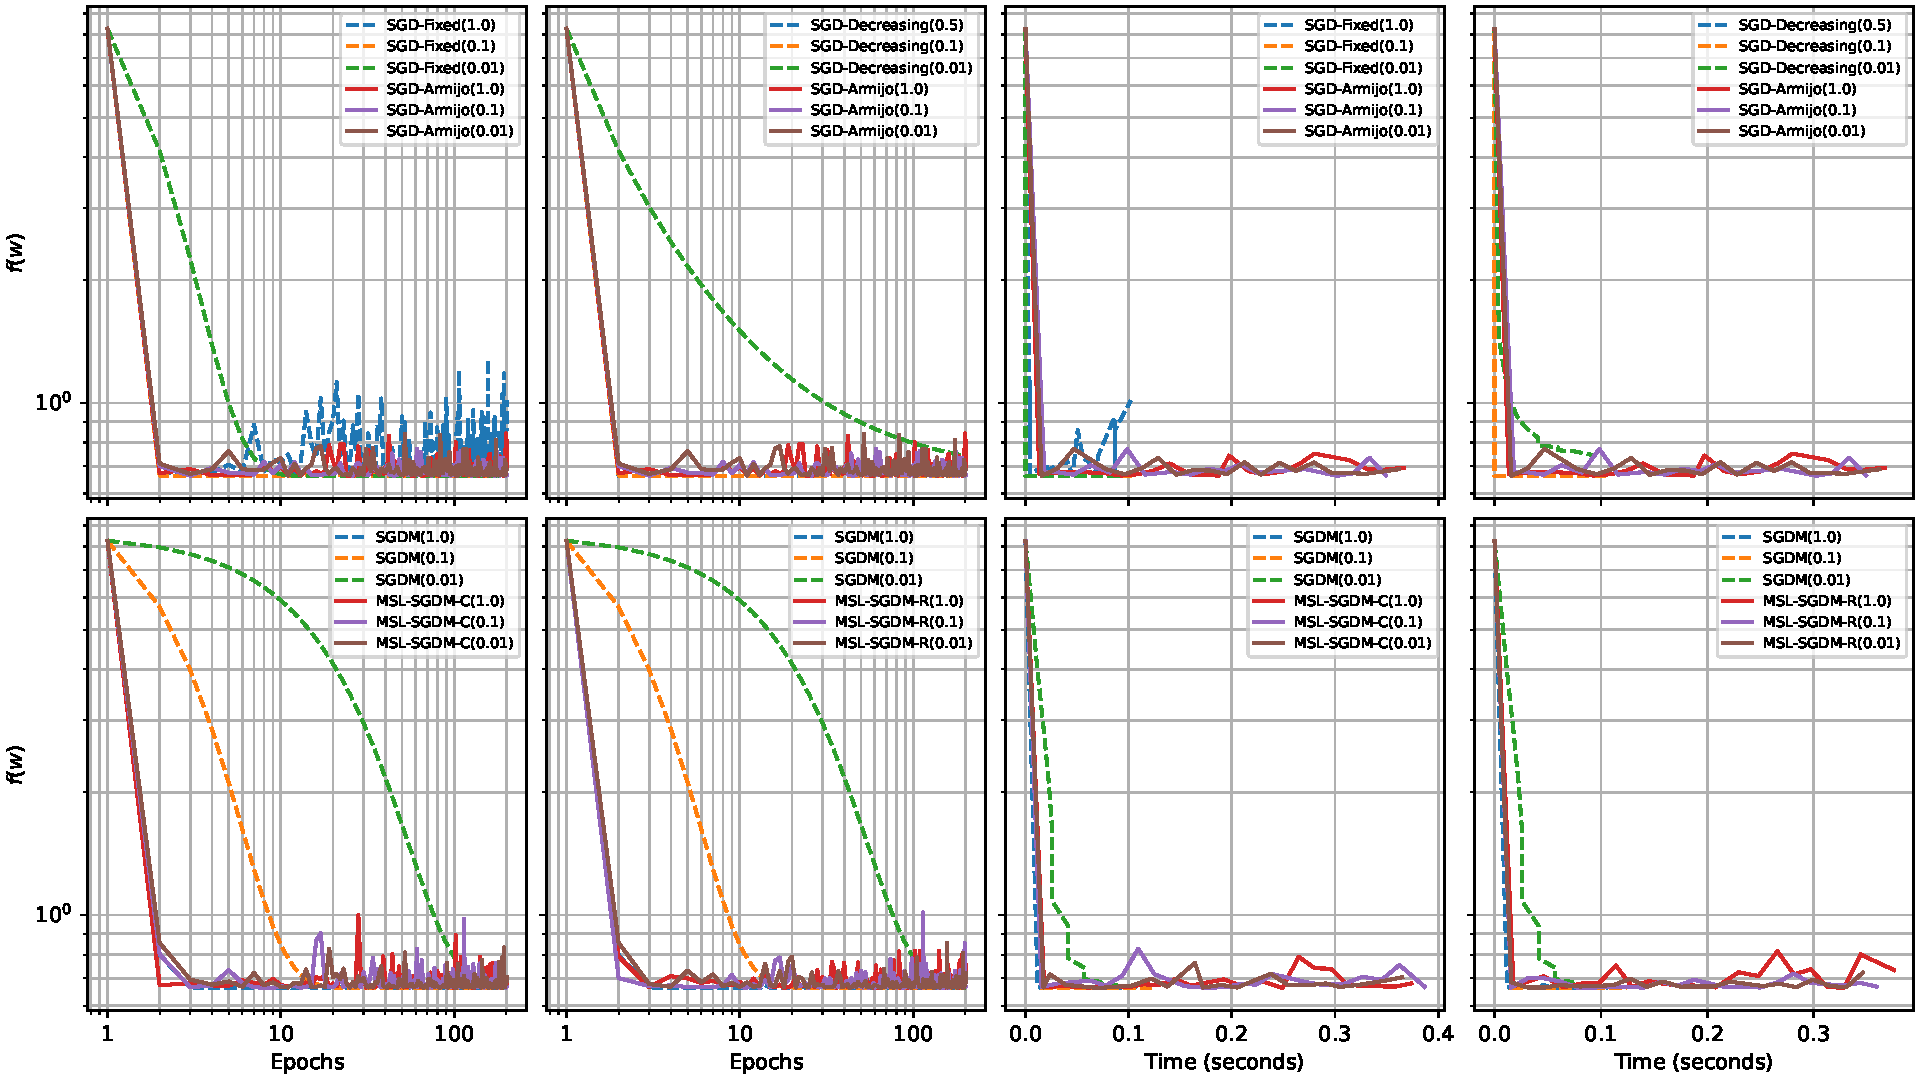
\includegraphics[width=\textwidth]{diab-diagnostic}} \\
% breast cancer
\subfloat[][\emph{Breast cancer dataset}\label{subfig:breast-diagnostic}]%
	{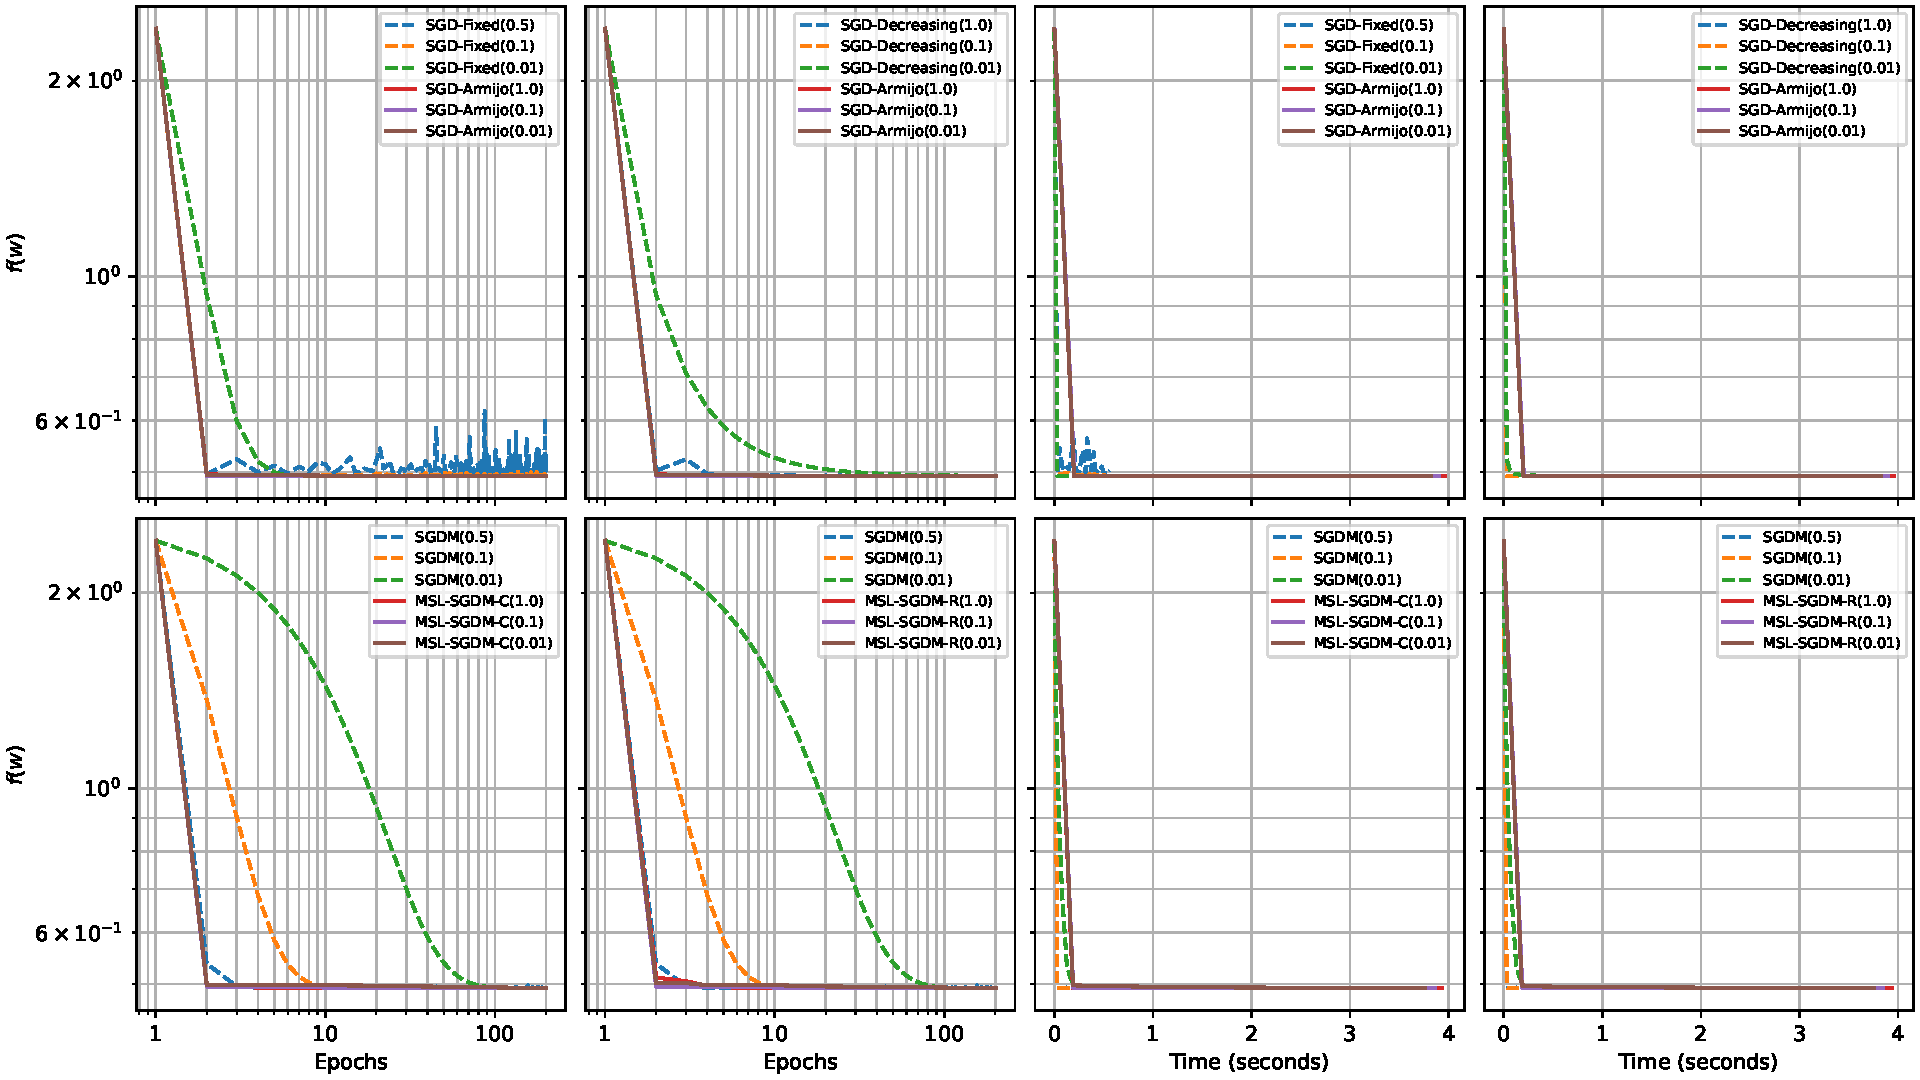
\includegraphics[width=\textwidth]{breast-diagnostic}} \\
\caption[]{Diabetes and Breast cancer}
\label{fig:diab-breast}
\end{figure}

\begin{figure}
\centering
% svmguide1
\subfloat[][\emph{svmguide1 dataset}\label{subfig:svm-diagnostic}]%
	{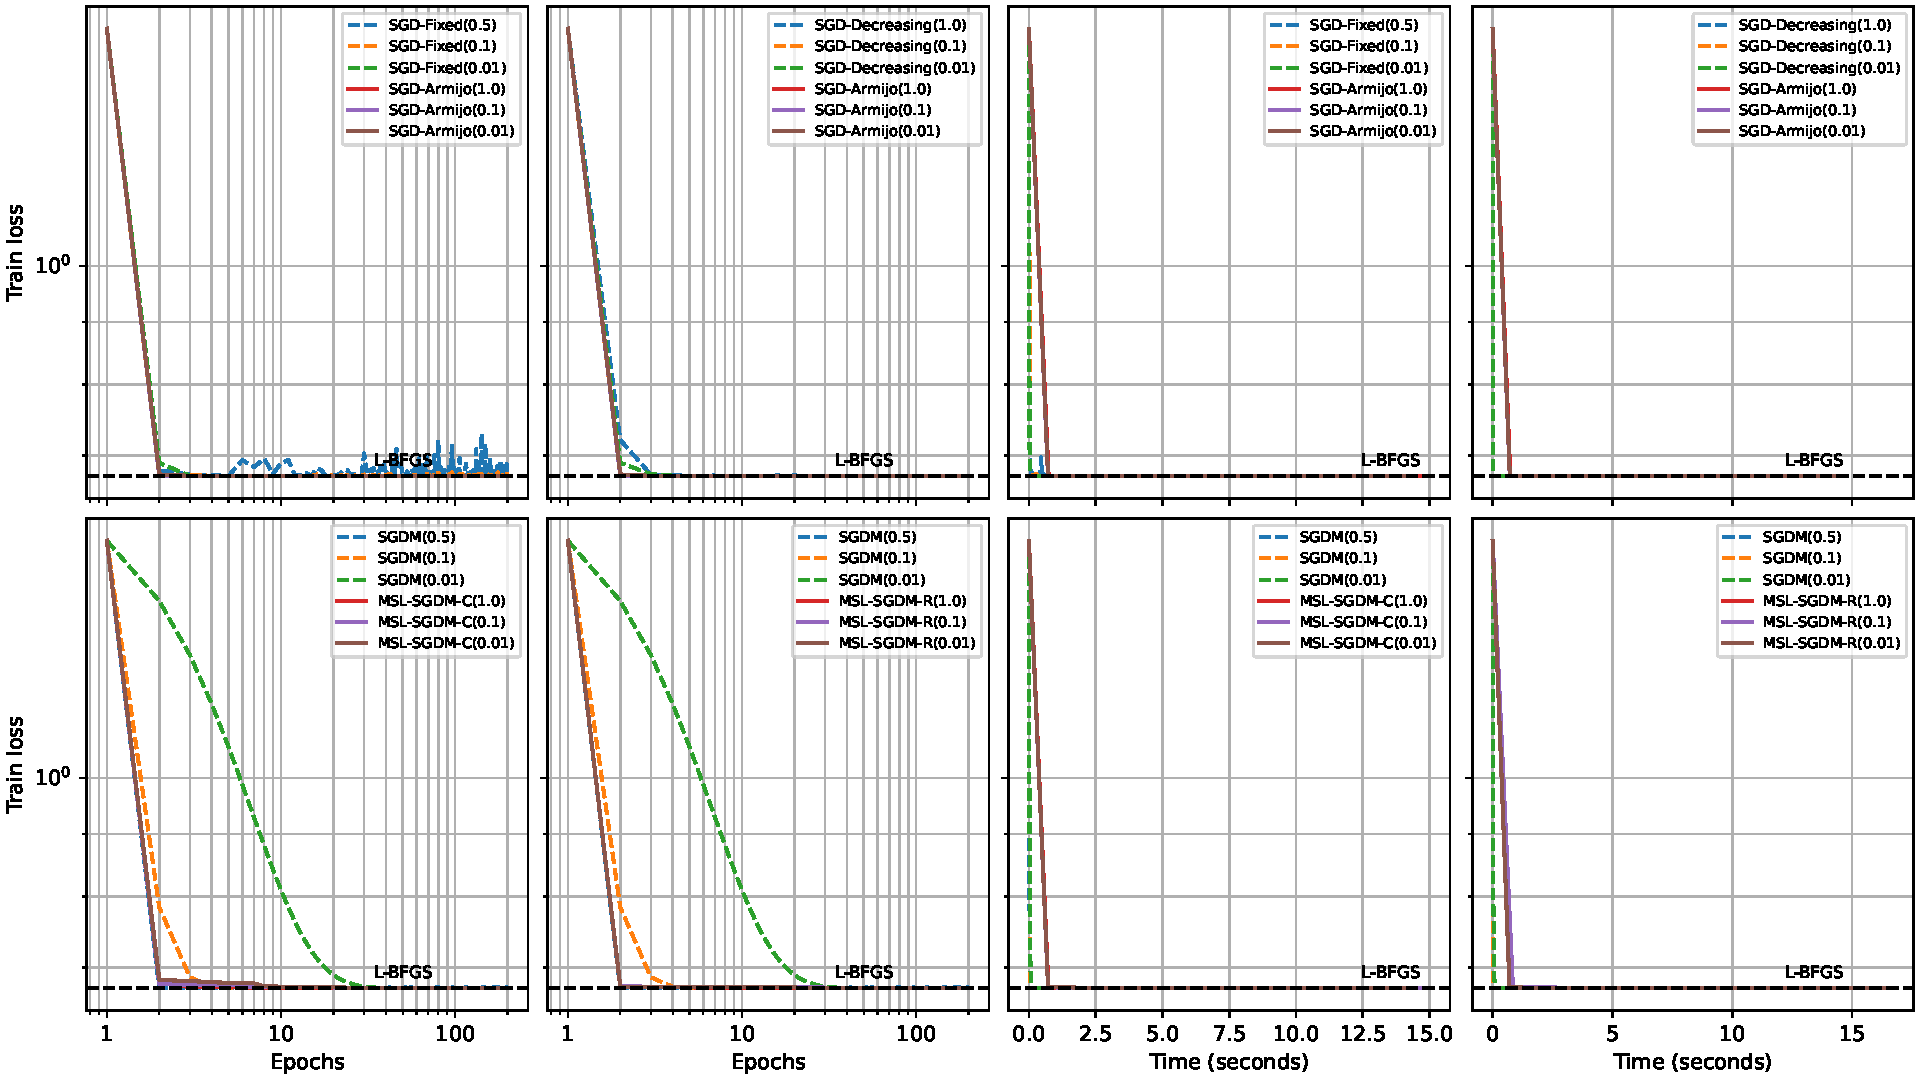
\includegraphics[width=\textwidth]{svm-diagnostic}} \\
% australian
\subfloat[][\emph{Australian dataset}\label{subfig:austr-diagnostic}]%
	{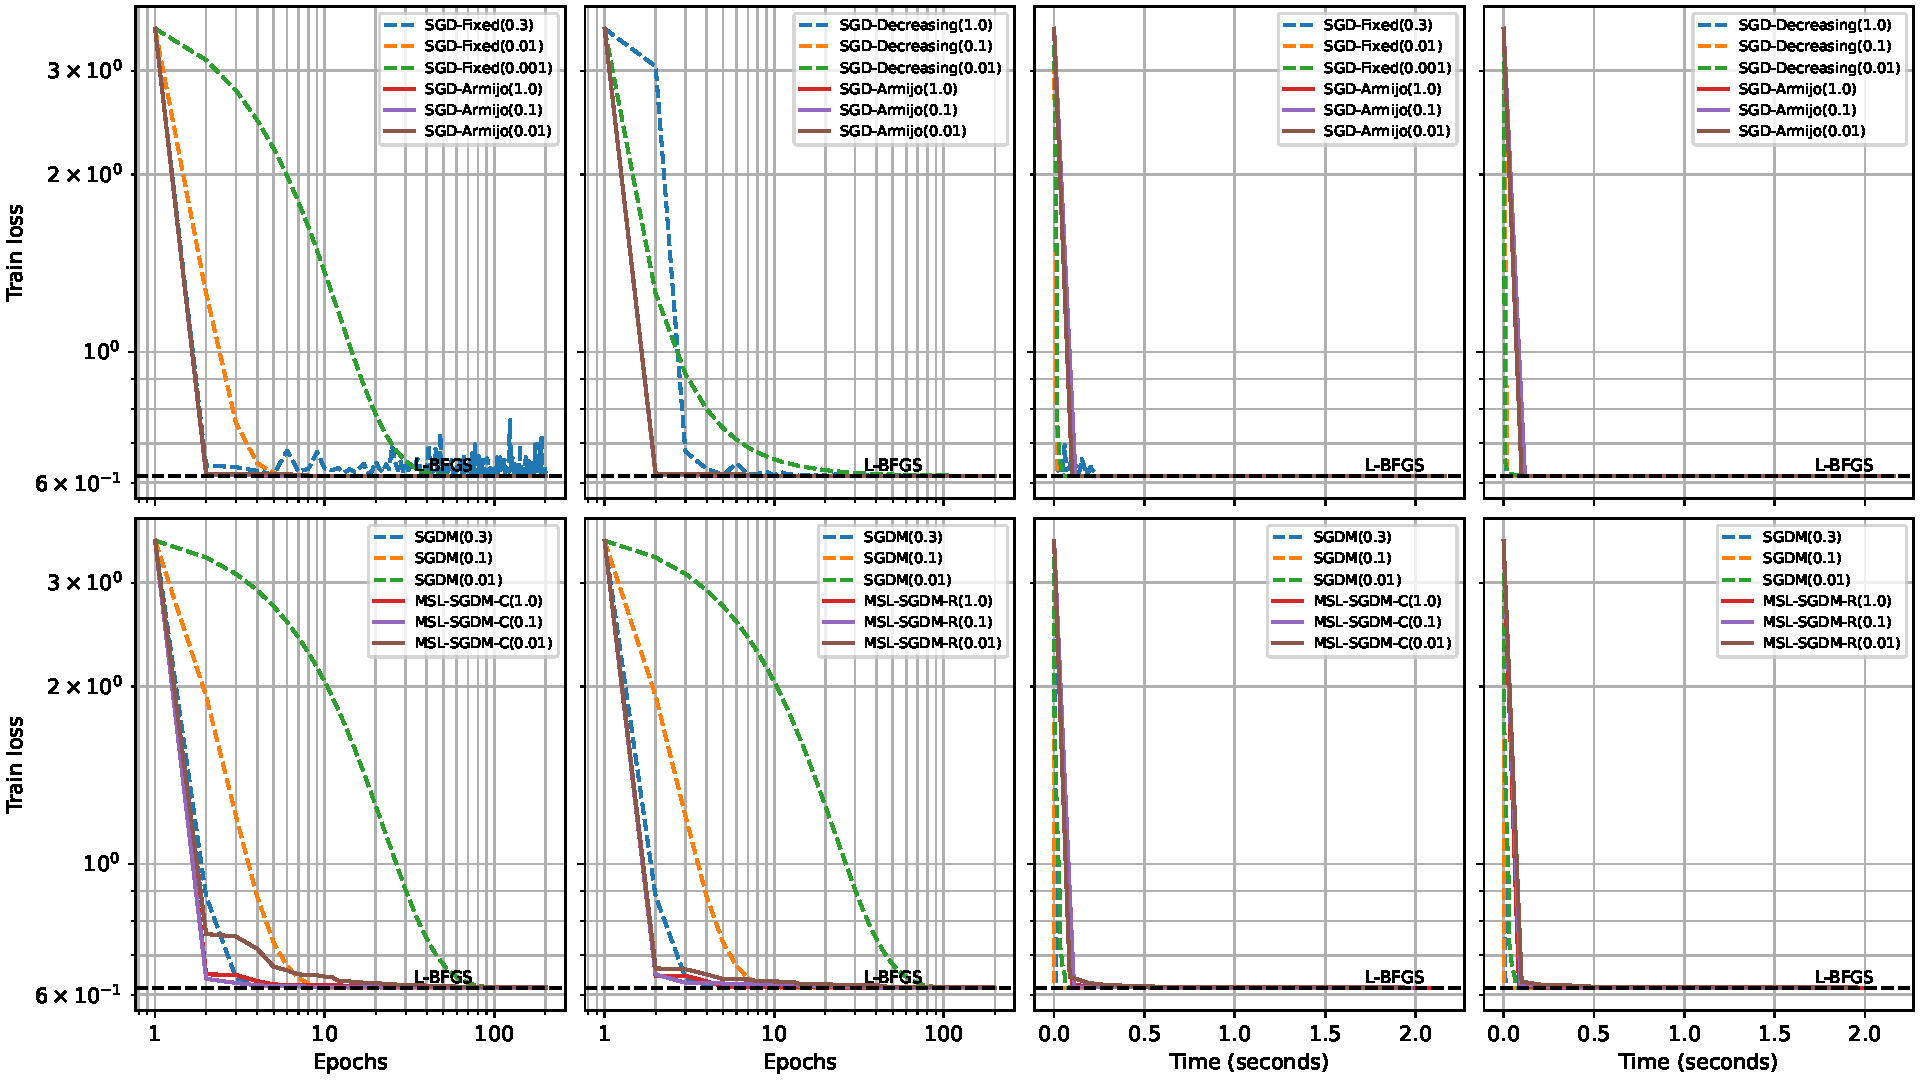
\includegraphics[width=\textwidth]{austr-diagnostic}}
\caption[]{svmguide1 and Australian datasets}
\label{fig:svm-austr}
\end{figure}

\begin{figure}
\centering
% mushrooms
\subfloat[][\emph{Mushrooms dataset}\label{subfig:mush-diagnostic}]%
	{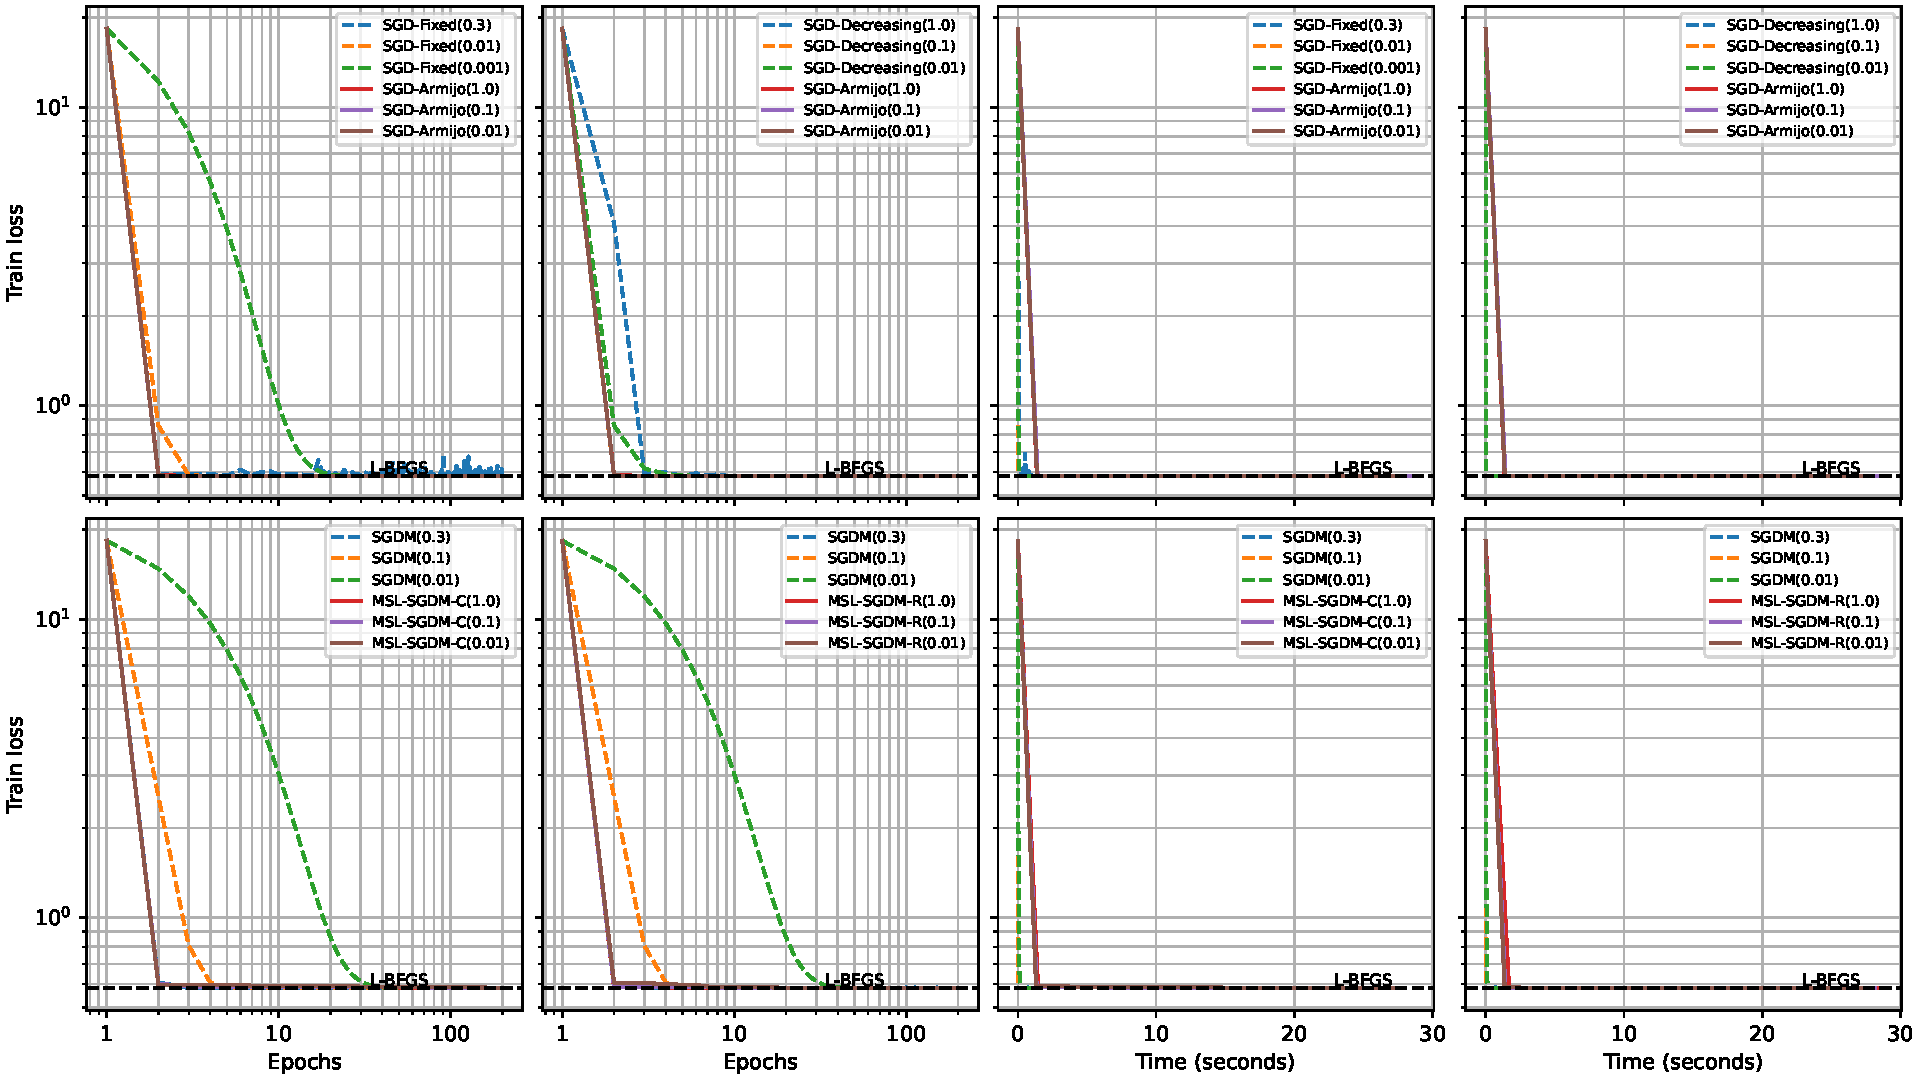
\includegraphics[width=\textwidth]{mush-diagnostic}} \\
% german
\subfloat[][\emph{German dataset}\label{subfig:german-diagnostic}]%
	{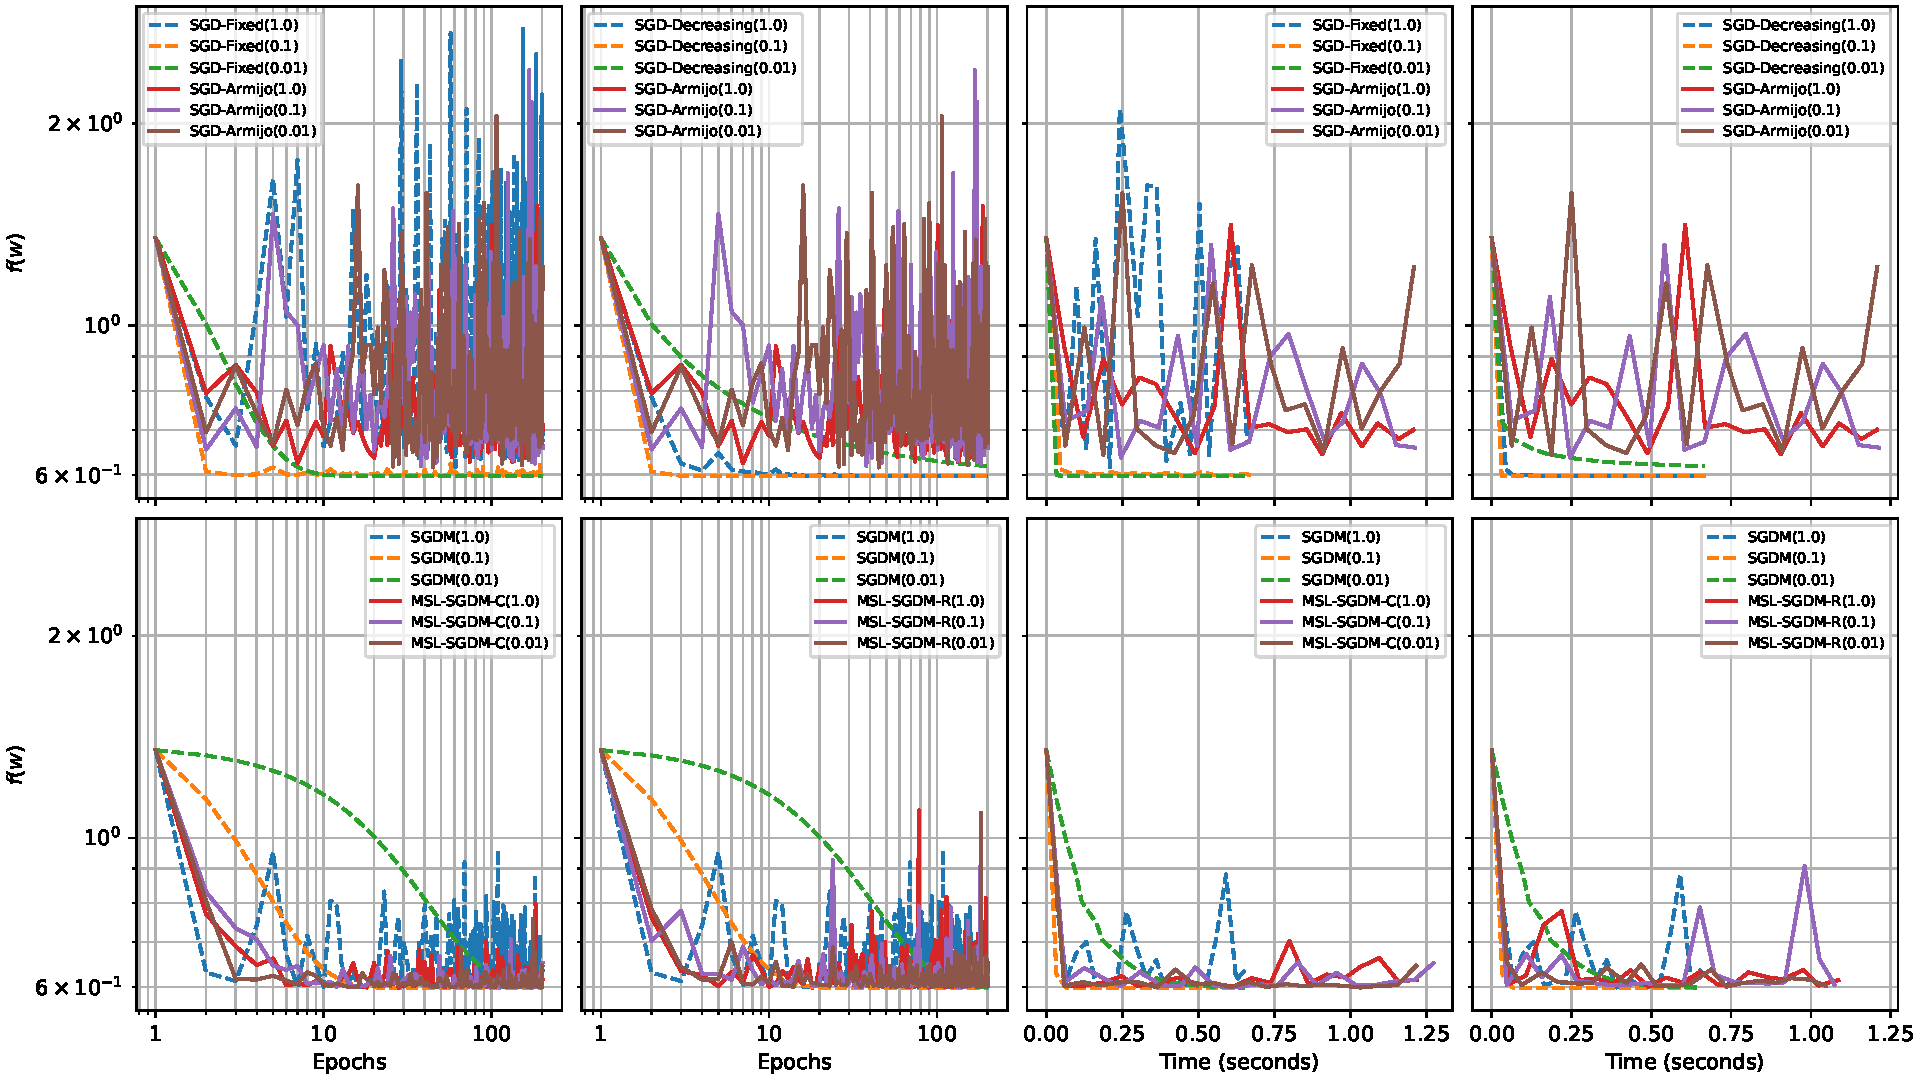
\includegraphics[width=\textwidth]{german-diagnostic}}
\caption[]{Mushrooms and German datasets}
\label{fig:mush-german}
\end{figure}


\begin{table}
\sisetup{round-mode=places}
\centering
\caption{Diabetes dataset}
\label{tab:diab-table}
\begin{tabular}{lS[round-precision=3]S[drop-zero-decimal]S[round-precision=4]S[round-precision=6]S[round-precision=4]}
\toprule
Solver & {$\alpha_0$} & {Epochs} & {Run-time} & {Loss} & {Test score} \\
\midrule
Newton-CG & NaN & 5 & NaN & 0.662128 & 0.642857 \\
CG & NaN & 6 & NaN & 0.662128 & 0.642857 \\
L-BFGS & NaN & 6 & NaN & 0.662128 & 0.642857 \\
SGD-Fixed & 0.005000 & 25 & 0.000000 & 0.662128 & 0.642857 \\
MSL-SGDM-R & 0.800000 & 186 & 0.000000 & 0.662129 & 0.642857 \\
SGDM & 0.050000 & 38 & 0.000000 & 0.662129 & 0.642857 \\
SGD-Armijo & 0.500000 & 98 & 0.000000 & 0.662129 & 0.642857 \\
SGD-Decreasing & 1.000000 & 101 & 0.000000 & 0.662129 & 0.642857 \\
MSL-SGDM-C & 0.100000 & 200 & 3.682196 & 0.662188 & 0.642857 \\
\bottomrule
\end{tabular}
\end{table}

\begin{table}
\sisetup{round-mode=places}
\centering
\caption{Breast cancer dataset}
\label{tab:breast-tab}
\begin{tabular}{lS[round-precision=3]S[drop-zero-decimal]S[round-precision=4]S[round-precision=6]S[round-precision=4]}
\toprule
Solver & {$\alpha_0$} & {Epochs} & {Run-time} & {Loss} & {Test score} \\
\midrule
Newton-CG & NaN & 7 & NaN & 0.492561 & 0.817518 \\
CG & NaN & 8 & NaN & 0.492561 & 0.817518 \\
L-BFGS & NaN & 7 & NaN & 0.492561 & 0.817518 \\
SGDM & 0.050000 & 76 & 0.000000 & 0.492561 & 0.817518 \\
SGD-Fixed & 0.005000 & 24 & 0.492562 & 0.492561 & 0.817518 \\
SGD-Decreasing & 1.000000 & 129 & 0.000000 & 0.492561 & 0.817518 \\
SGD-Armijo & 1.000000 & 81 & 0.000000 & 0.492562 & 0.817518 \\
MSL-SGDM-R & 0.500000 & 200 & 3.229806 & 0.492572 & 0.817518 \\
MSL-SGDM-C & 0.500000 & 200 & 3.264365 & 0.492730 & 0.817518 \\
\bottomrule
\end{tabular}
\end{table}

\begin{table}
\sisetup{round-mode=places}
\caption{svmguide1 dataset}
\label{tab:svm-tab}
\centering
\begin{tabular}{lS[round-precision=3]S[drop-zero-decimal]S[round-precision=4]S[round-precision=6]S[round-precision=4]}
\toprule
Solver & {$\alpha_0$} & {Epochs} & {Run-time} & {Loss} & {Test score} \\
\midrule
Newton-CG & NaN & 5 & NaN & 0.673302 & 0.516750 \\
CG & NaN & 8 & NaN & 0.673302 & 0.516750 \\
L-BFGS & NaN & 5 & NaN & 0.673302 & 0.516250 \\
SGD-Fixed & 0.010000 & 24 & 0.000000 & 0.673303 & 0.517250 \\
SGDM & 0.050000 & 15 & 0.000000 & 0.673303 & 0.517000 \\
SGD-Decreasing & 1.000000 & 56 & 0.000000 & 0.673303 & 0.517000 \\
SGD-Armijo & 0.500000 & 21 & 0.000000 & 0.673303 & 0.515500 \\
MSL-SGDM-R & 1.000000 & 193 & 0.000000 & 0.673304 & 0.516000 \\
MSL-SGDM-C & 0.100000 & 200 & 14.715103 & 0.673363 & 0.508500 \\
\bottomrule
\end{tabular}
\end{table}


\begin{table}
\sisetup{round-mode=places}
\caption{Australian dataset}
\label{tab:austr-tab}
\centering
\begin{tabular}{lS[round-precision=3]S[drop-zero-decimal]S[round-precision=4]S[round-precision=6]S[round-precision=4]}
\toprule
Solver & {$\alpha_0$} & {Epochs} & {Run-time} & {Loss} & {Test score} \\
\midrule
Newton-CG & NaN & 7 & NaN & 0.615582 & 0.876812 \\
L-BFGS & NaN & 7 & NaN & 0.615582 & 0.876812 \\
CG & NaN & 8 & NaN & 0.615582 & 0.876812 \\
SGD-Decreasing & 0.050000 & 18 & 0.000000 & 0.615582 & 0.876812 \\
SGDM & 0.020000 & 190 & 0.000000 & 0.615582 & 0.876812 \\
SGD-Fixed & 0.001000 & 108 & 0.000000 & 0.615582 & 0.876812 \\
SGD-Armijo & 0.700000 & 200 & 4.442389 & 0.615585 & 0.876812 \\
MSL-SGDM-R & 1.000000 & 200 & 4.459376 & 0.615638 & 0.884058 \\
MSL-SGDM-C & 1.000000 & 200 & 4.499516 & 0.615716 & 0.876812 \\
\bottomrule
\end{tabular}
\end{table}


\begin{table}
\sisetup{round-mode=places}
\caption{Mushrooms dataset}
\label{tab:mush-tab}
\centering
\begin{tabular}{lS[round-precision=3]S[drop-zero-decimal]S[round-precision=4]S[round-precision=6]S[round-precision=4]}
\toprule
Solver & {$\alpha_0$} & {Epochs} & {Run-time} & {Loss} & {Test score} \\
\midrule
Newton-CG & NaN & 8 & NaN & 0.580925 & 0.886154 \\
L-BFGS & NaN & 9 & NaN & 0.580925 & 0.886154 \\
CG & NaN & 10 & NaN & 0.580925 & 0.886154 \\
SGD-Fixed & 0.001000 & 45 & 0.000000 & 0.580925 & 0.886154 \\
SGDM & 0.010000 & 92 & 2.098158 & 0.580925 & 0.886154 \\
SGD-Decreasing & 0.100000 & 54 & 0.000000 & 0.580925 & 0.886154 \\
SGD-Armijo & 1.000000 & 200 & 58.344068 & 0.580938 & 0.886154 \\
MSL-SGDM-R & 1.000000 & 200 & 58.148211 & 0.581116 & 0.884923 \\
MSL-SGDM-C & 1.000000 & 200 & 58.191985 & 0.581724 & 0.887385 \\
\bottomrule
\end{tabular}
\end{table}


\begin{table}
\sisetup{round-mode=places}
\caption{German dataset}
\label{tab:german-tab}
\centering
\begin{tabular}{lS[round-precision=3]S[drop-zero-decimal]S[round-precision=4]S[round-precision=6]S[round-precision=4]}
\toprule
Solver & {$\alpha_0$} & {Epochs} & {Run-time} & {Loss} & {Test score} \\
\midrule
Newton-CG & NaN & 7 & NaN & 0.619120 & 0.700000 \\
L-BFGS & NaN & 10 & NaN & 0.619120 & 0.700000 \\
CG & NaN & 9 & NaN & 0.619120 & 0.700000 \\
SGD-Decreasing & 1.000000 & 161 & 0.000000 & 0.619120 & 0.700000 \\
SGD-Fixed & 0.005000 & 63 & 0.000000 & 0.619121 & 0.700000 \\
SGD-Armijo & 1.000000 & 200 & 1.596410 & 0.619132 & 0.700000 \\
SGDM & 0.025000 & 200 & 0.165398 & 0.619138 & 0.700000 \\
MSL-SGDM-R & 1.000000 & 200 & 1.602347 & 0.619192 & 0.700000 \\
MSL-SGDM-C & 1.000000 & 200 & 1.597145 & 0.619393 & 0.700000 \\
\bottomrule
\end{tabular}
\end{table}




%\cleardoublepage
% ***************************************************** %
%\section{Mathematical background}
% ***************************************************** %

%\begin{defs}[Convex function]\label{def:conv_fun}
%	Let $S\subseteq\R^n$ be a convex set, a function $f\colon S\to\R$ is said to be convex if the hessian matrix is semi-positive-defined. If the hessian matrix is positive-defined, then the function is strictly convex.
%\end{defs}
%
%\begin{thm}[Weirstrass theorem]\label{thm:weirs}
%	Let $f\colon\R^n\to\R$ be a continuous function and $S\subseteq\R^n$ a compact set. Then function $f$ admits global minimum in $S$.
%\end{thm}
%
%\begin{cor}[Sufficient condition]\label{cor:weirs1}
%	If function $f\colon\R^n\to\R$ is a continuous and coercive function, then $f$ admits global minimum in $\R^n$.
%\end{cor}
%
%\begin{prop}[Coercivity of a quadratic function]
%	A quadratic function $\func(x)=\frac{1}{2}x^TQx-c^Tx$ is said to be coercive if and only if the symmetric matrix $Q\in\R^{n\times n}$ is positive-defined.
%\end{prop}
%
%\begin{prop}[Unique global minimum]\label{prop:min_unique}
%	Let $S\subseteq\R^n$ be a convex set, let $f\colon S\to\R$ be a strictly convex function. Then the global minimum, if exists, is unique.
%\end{prop}
%
%\begin{prop}[First order optimality condition]
%	$\bar{x}$ is a local minimum for $f\colon\R^n\to\R$ of class $f\in C^1(\R^n)$ if and only if $\nabla\func(\bar{x})=0$.
%\end{prop}
%
%\begin{prop}[Second order optimality condition]\label{prop:opt_second}
%	$\bar{x}\in\R^n$ is a local minimum for $f\colon\R^n\to\R$ of class $f\in C^2(\R^n)$ if and only if
%	\[\nabla\func(\bar{x})=0\quad\wedge\quad \nabla^2\func(\bar{x})\,\,\,\text{positive semi-definite}\]
%\end{prop}

% add definition of coercive function and proposition about compact sets?
% add gradient descent?
